%%%%%%%%%%%%%%%%%%%%%%%%%%%%%%%%%%%%%%%%%%%%%%%%%%%%%%%%%%%%%%%%%%% 
%                                                                 %
%                            CHAPTER                              %
%                                                                 %
%%%%%%%%%%%%%%%%%%%%%%%%%%%%%%%%%%%%%%%%%%%%%%%%%%%%%%%%%%%%%%%%%%% 

\chapter{Achtergrond}

\section{Fitnesstrackers}
Zoals al enkele malen werd aangehaald ligt de focus van deze scriptie op
mogelijke tekortkomingen/vulnerabilities betreffende privacybeleid in
fitnesstrackers. Maar voordat een aanval kan worden opgezet, is het
noodzakelijk om een te vat te krijgen op welke manier een fitnesstracker info
verzamelt en weergeeft, en meer precies, hoe de mechanismen die de privacy
voorzien voor de gebruikers in detail werken. Dit is essentiële informatie om
een aanval te kunnen opzetten.

De gebruikte data waarop de aanval wordt opgezet en waar op wordt
geëxperimenteerd, is afkomstig van de populaire fitnesstracker
\textit{Strava\footnote{\url{https://www.strava.com/}}}. Dit is een sociaal
netwerk, waarbij een alle soorten sporters hun activiteiten kunnen delen. Dit
gaat over lopen, wandelen, fietsen, zwemmen, \ldots, maar ook sporten als
fitnessen, voetballen, \ldots (Deze laatste zijn wel veruit in de minderheid
bij de overschouwing van de totale verdeling van alle
activiteiten\cite{Stravas24:online}). De betreffende data wordt in perspectief
van een mogelijke aanval gefilterd, opdat enkel activiteiten die relevante
gps-informatie bevatten in beschouwing worden genomen. Dit gaat dan meer
specifiek over \textit{runs, hikes, walks, and rides}.

\subsection{Activiteiten}
Een Strava activiteit bevat erg veel informatie. Echter is niet alles even
bruikbaar. Een correcte abstractie zal dus moeten gemaakt worden van de
onnodige data. Afbeelding~\ref{fig:activityData} geeft een voorbeeld van een
gedetailleerde activiteit weer. Een gebruiker is in staat om de activiteit een
titel te geven, en er een korte beschrijving aan toe te voegen. Ook een foto
kan optioneel toegevoegd worden. De exacte datum en tijd van de start van de
activiteit wordt hierbij ook weergegeven.

Rechts daarvan zijn de algemene basisstatistieken te zien. Deze zijn de totale
afgelegde afstand, de totale bewegingstijd, de gemiddelde snelheid, het totale
hoogteverschil, de totale verstreken tijden het aantal calorieën verbrand. Als
extra kunnen hier enkele statistieken m.b.t.\ het gebruikte materiaal, zoals
type fiets, loopschoenen, hartslagmeter, enzovoort worden weergegeven. Een
belangrijk onderscheid in deze context is het verschil tussen de beweegtijd en
de verstreken tijd. Deze 2 lijken in definitie gelijk, maar dit zijn ze niet!
Strava werkt met 2 verschillende soorten tijdsberekeningen voor een iets
accuratere snelheidsberekening. De verstreken tijd is simpelweg het
tijdsinterval tussen het vertrek van de activiteit en de aankomsttijd ervan. De
bewegingstijd is de tijd waarbij de gebruiker zich effectief bewoog. M.a.w.
worden de tijden waarbij de gebruiker stilstond uit de verstreken tijd
gefilterd. Dit kan gaan over bijvoorbeeld een pauze, of een verkeerslicht. De
snelheid wordt berekend aan de hand van de bewegingstijd. Dit kan simpel worden
geverifieerd worden via een manuele berekening ter bevestiging(\ref{eq:speed}).
Een kanttekening hierbij is dat dit enkel geldt voor activiteiten die niet
gelabeld zijn als \textit{race}. In dit geval wordt de snelheid berekend in
functie van de totaal verstreken tijd.\cite{MovingTi80:online}
\begin{equation}\label{eq:speed}
    \frac{(39:17)\min}{7.44 km} = 5:16 \min
\end{equation}

Daaronder zien we de \textit{Strava-segmenten}. Een Strava-segment is een
specifiek deel van een bepaalde route dat door gebruikers van de sport-app kan
worden gemarkeerd, gedeeld en vergeleken met andere gebruikers. Het segment is
een bepaalde afstand en route, bijvoorbeeld een klim of afdaling, die vaak
wordt beschouwd als een uitdagende of iconische sectie van een bepaalde fiets-
of hardlooproute. Gebruikers van Strava kunnen een segment maken door de begin-
en eindpunten op een kaart aan te geven en een naam en beschrijving toe te
voegen. Zodra het segment is gemaakt, kunnen andere gebruikers het segment
vinden en deelnemen aan een leaderboard, waarop de snelste tijden worden
bijgehouden en vergeleken met andere gebruikers. Segmenten worden vaak gebruikt
om prestaties te meten en te vergelijken.

Daarnaast is ook de kaart duidelijk zichtbaar. Daarbij horen ook de
tussentijden en de grafiek van snelheid. Optioneel kan hierbij ook nog een
grafiek van de afgelegde hoogte en de hartslag worden weergegeven, indien de
gebruiker hiervoor met het juiste materieel zijn sportactiviteit opneemt. De
tussentijden en de grafiek van snelheid zijn qua inhoud gelijkaardig, met als
verschil dat de grafiek erg precies kan worden bestudeerd worden. Op de grafiek
is voor elk afstandspunt de ogenblikkelijke snelheid zichtbaar. Bij de
tussentijden is wordt de gemiddelde snelheid over een kilometer weergegeven. De
kaart die de route weergeeft is zeker ook belangrijk om even te bestuderen.
Deze bevat namelijk alle gps-geregistreerde punten, en verbindt deze ook om zo
één aaneensluitende route te vormen. Wanneer deze echter in detail bestudeerd
wordt, samen met de legende die aanwezig is, is te zien dat de route uit twee
delen bestaat, een zichtbaar deel en een onzichtbaar deel. Dit heeft betrekking
tot wat zichtbaar is voor een andere gebruiker die deze activiteit bekijkt.
Deze gebruiker zal enkel zicht hebben tot de het zichtbare deel, het
onzichtbare deel zal dus voor een andere gebruiker niet zichtbaar zijn. De
activiteit zal voor deze persoon dus als het ware afgekapt zijn, en zal in zijn
zichtbare versie op een andere plek starten en eindigen. In de volgende
sectie~\ref{Algemene Privacy} \&~\ref{EPZ} wordt op de betekenis meer in detail
ingegaan op de werking van deze methodiek.

Een laatste kanttekening die hierbij gemaakt moet worden is dat voor een
gebruiker verschillende eenheden mogelijk zijn om uit te kiezen. Er is keuze
mogelijk tussen de mijl en pond, en kilometer en kilogram. Een gebruiker kiest
in welke eenheid hij/zij de applicatie wenst te gebruiken. Voor de gebruiker in
kwestie zal dus alles worden weergegeven in de gekozen eenheid.
\begin{figure}
    \centering
    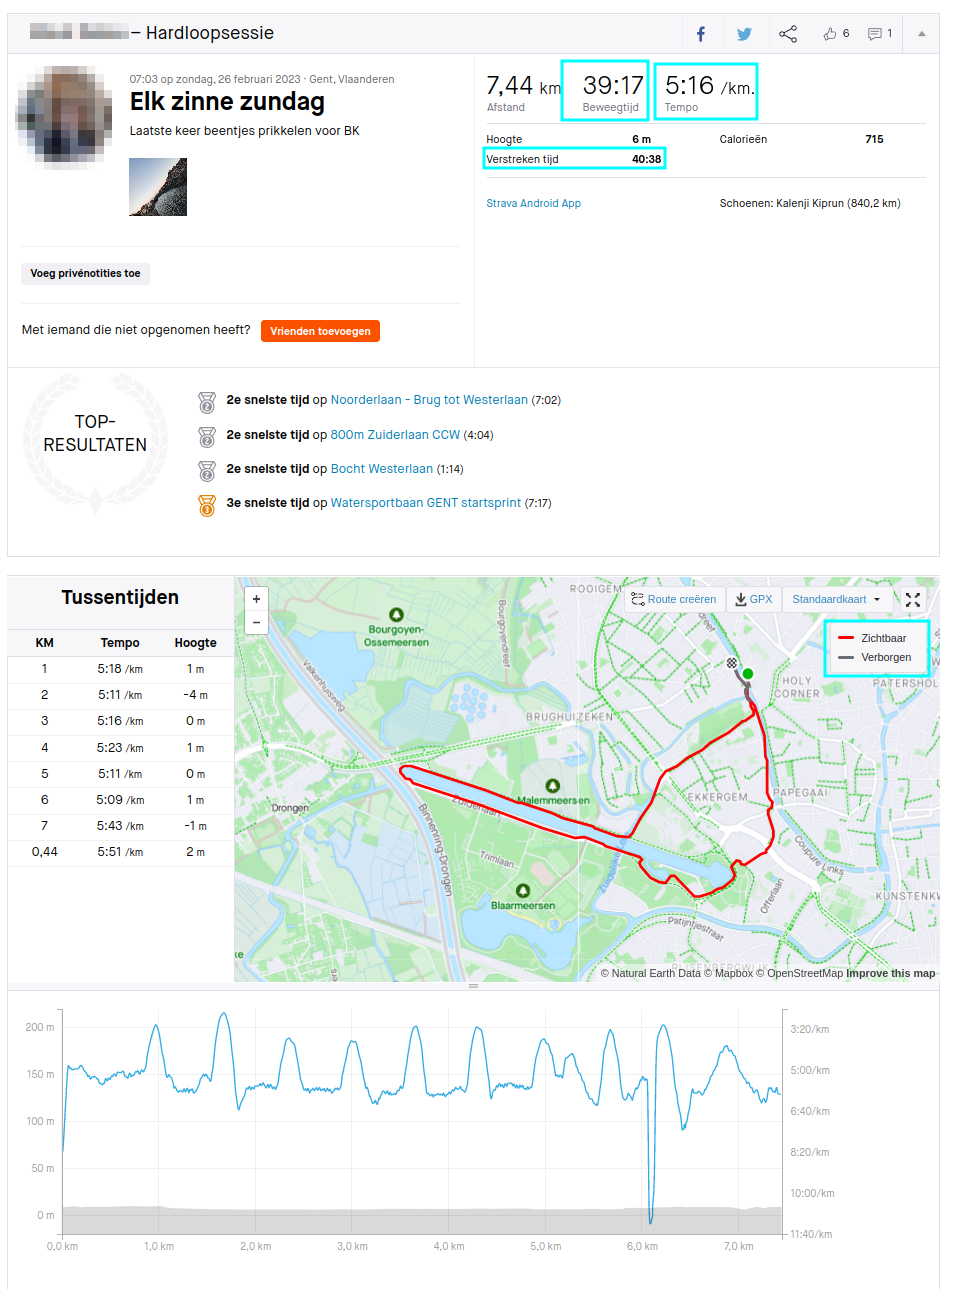
\includegraphics[width=0.8\textwidth]{fig/VoorbeeldActiviteit_Personal.png}
    \caption{Data van een activiteit}\label{fig:activityData}
\end{figure}

\subsection{Algemene Privacy}\label{Algemene Privacy}
Het delen van alle data die vervat zit in zo'n een activiteit zit met alle
andere gebruikers op het platform, is zeker niet altijd wenselijk. Kiezen er
dan ook voor om de gebruiker de mogelijkheid te geven om zijn privacy te
verbeteren. In deze sectie wordt de focus gelegd op de mechanismen in gebruikt
in \textit{Strava}, maar in heel wat andere sport-applicaties worden
vergelijkbare, zo niet dezelfde methodieken gebruikt.

\subsection{Endpoint Privacy Zones}\label{EPZ}